\chapter{Практические задания}
\section{Задание №1}
\textbf{Задание:} составить базу знаний <<Предки>>, позволяющую наиболее эффективным способом (за меньшее количество шагов, что обеспечивается меньшим количеством предложений в БЗ -- правил), используя разные варианты (примеры) одного вопроса, определить (указать, какой вопрос для какого варианта):
\begin{enumerate}
	\item по имени субъекта определить всех его бабушек (предки 2-ого колена);
	\item по имени субъекта определить всех его дедушек (предки 2-ого колена);
	\item по имени субъекта определить всех его бабушек и дедушек (предки 2-ого колена);
	\item по имени субъекта определить его бабушку по материнской линии (предки 2-ого колена);
	\item по имени субъекта определить его бабушку и дедушку по материнской линии (предки 2-ого колена);
\end{enumerate}
Минимизировать количество правил и количество вариантов вопросов. Использовать конъюнктивные правила и простой вопрос.

Для одного из вариантов вопроса и конкретной БЗ составить таблицу, отражающую конкретный порядок работы системы, с объяснениями:
\begin{itemize}
	\item очередная проблема на текущем шаге и метод решения;
	\item каково новое текущее состояние резольвенты, как получено;
	\item какие дальнейшие действия? (запускается ли алгоритм унификации? Каких термов? Почему этих?);
	\item вывод по результатам очередного шага и дальнейшие действия.
\end{itemize}

Код программы представлен на листинге \ref{lst:code}.

\begin{lstlisting}[label=lst:code, basicstyle=\footnotesize, caption=Код программы]
domains
	sex = string
	name = symbol
	predicates
	parent(sex, name, name)
	grandparent(sex, name, name, sex)
clauses
	grandparent(Sex, Grandparent, Child_name, Line) :- parent(Line, Parent, Child_name), parent(Sex, GrandParent, Parent).
	
	parent("M", alexey, mark).
	parent("W", ulyana, mark).
	
	parent("W", julia, maria).
	parent("M", nikita, maria).
	
	parent("W", maria, rita).
	parent("W", maria, sasha).
	
	parent("M", roman, alexey).
	parent("W", tatiana, alexey).
	
	parent("W", sofia, ulyana).   
goal
	%Определить всех бабушек субъекта
	%grandparent("M", Grandparent, mark, _).
	
	%Определить всех его дедушек субъекта
	%grandparent("W", Grandparent, mark, _).
	
	%Определить всех бабушек и дедушек субъекта
	%grandparent(Sex, Grandparent, mark, Line).
	
	%Определить бабушку по материнской линии
	%grandparent("W", Grandparent, mark, "W").
	
	%Определить бабушку и дедушку по материнской линии
	%grandparent(Sex, Grandparent, rita, "W").
\end{lstlisting}

Ниже на рисунке \ref{image:table_1} приведена таблица порядка поиска ответа:
\begin{figure}[H]
	\centering{
		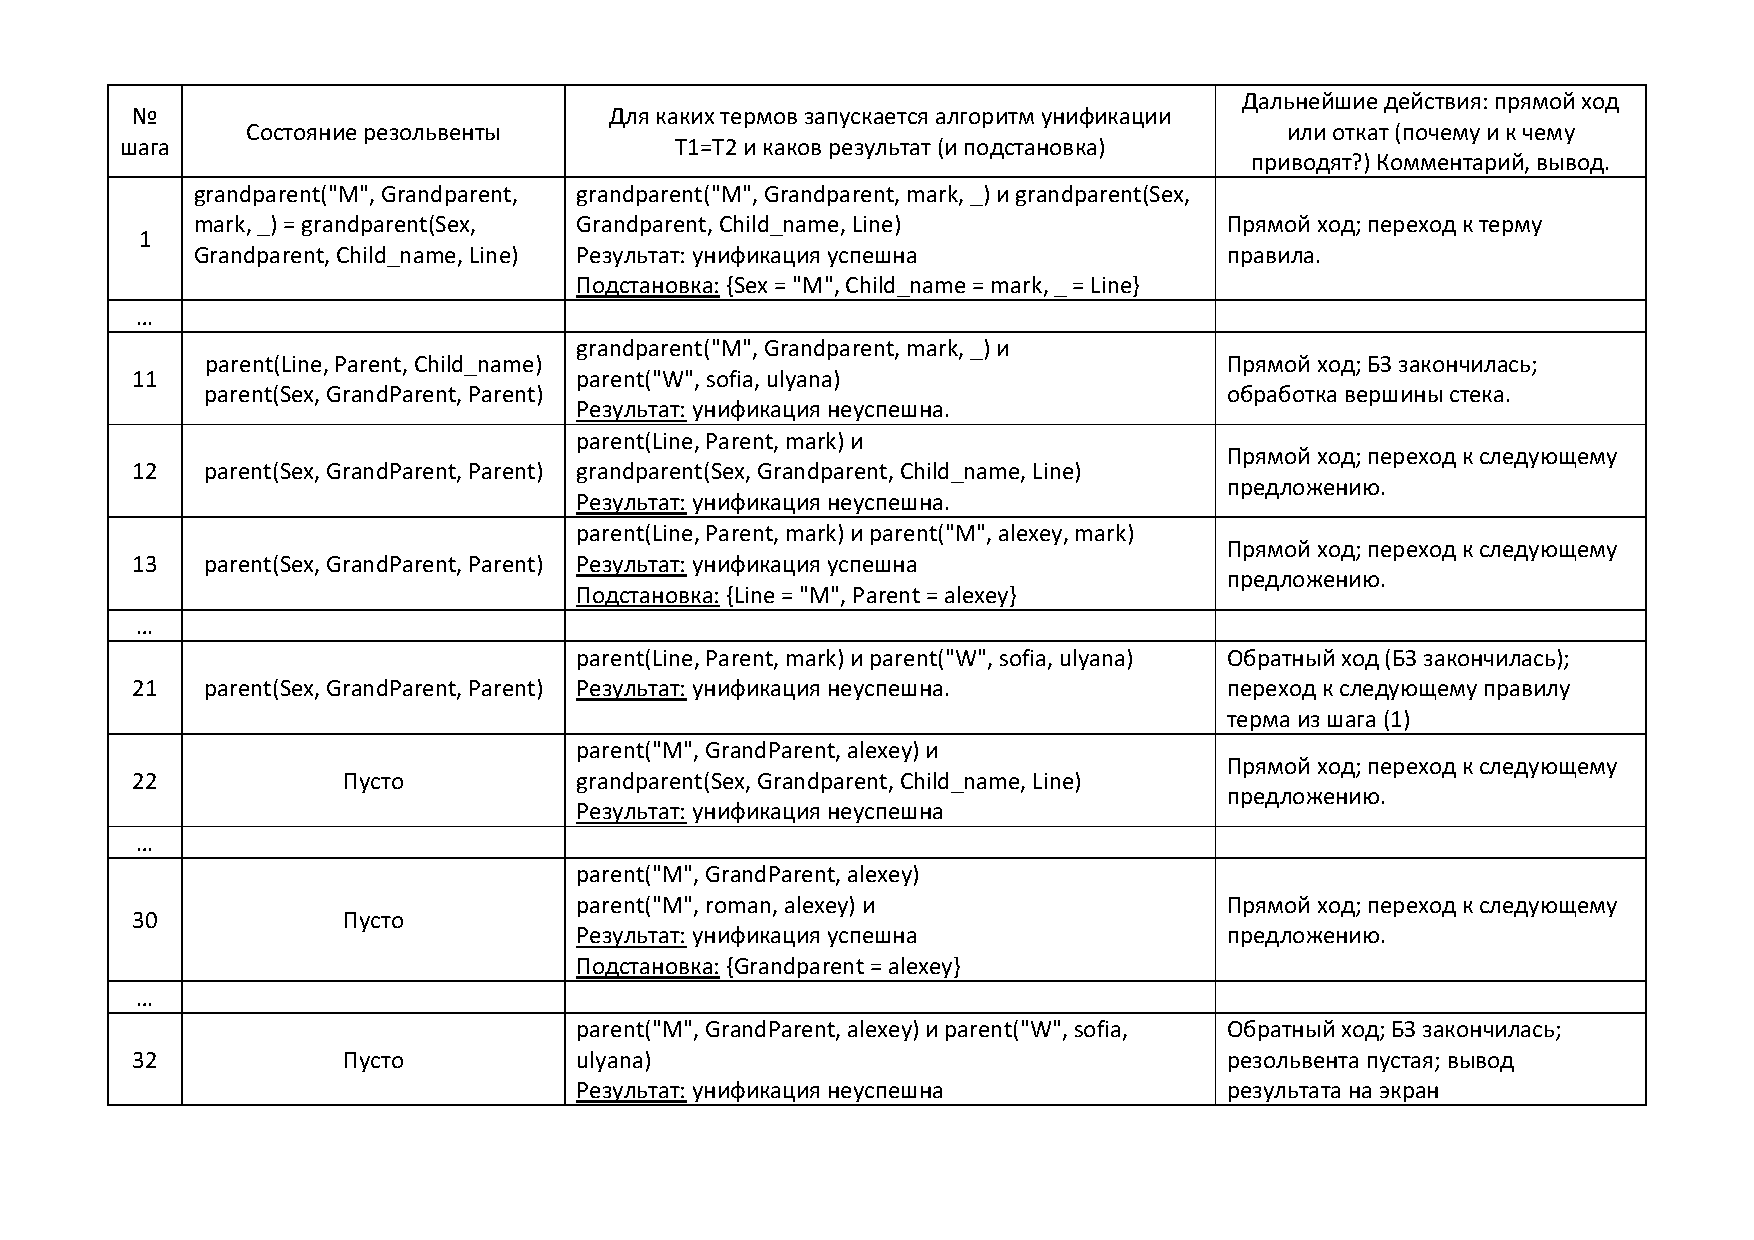
\includegraphics[scale=0.93, angle=90]{images/table_4.pdf}
		\caption{Таблица порядка поиска ответов.}
		\label{image:table_1}
	}
\end{figure}
